\chapter{Blockchain-Grundlagen}
\label{cha:grundlagen}

\section{Funktionsweise}
Die Funktionsweise der Blockchain wird hauptsächlich an Bitcoin erklärt. Als erste Blockchain-Anwendung \cite{ZhengBlockchainChallengesOpportunities2017} und aufgrund der relativ geringen Komplexität liefert es die Grundlage für die Funktion der Technologie. Andere Implementationen, wie Ethereum oder Ripple, funktionieren nach dem gleichen Prinzip.

%TODO: S.7 RavalDecentralized: The Problem that Blockchain solves about P2P
%TODO: S.1 Gramoli: Traditional Decentralisation to Blockchain
\subsection{Allgemein}
%TODO: Transaktionsgebühren erwähnen ? Oder erst in 5.1 ?
Wenn der Begriff ``Die Blockchain'' auftaucht, ist damit meistens die Blockchain-Technologie gemeint. Es gibt nicht nur eine global bestehende Blockchain und auch nicht nur eine Implementation der Technologie, was man an Bitcoin oder Ethereum sehen kann.

Allgemein kann man die Blockchain als Datenstruktur bezeichnen, welche verteilt, nicht löschbar und unmanipulierbar gespeichert werden kann. Weiterhin verifizieren jegliche Teilnehmer am Netzwerk ausgeführte Transaktionen, womit ein gemeinsamer Konsens über den Datenbestand besteht \cite{CrosbyBlockChainTechnologyBitcoin2016}.

%TODO: Speichert Fabric/Composer den Stand aller Daten ? Oder ergibt sich dieser aus den Transaktionen ? --> Siehe S.14 Scherer: Ledger and State Database
%TODO: Klarmachen das Daten in der Blockchain geändert werden können. Die alten Daten sind aber trotzdem noch einsehbar, da die Transaktion dazu in der Blockchain besteht
%TODO: Metadaten Beispiele nennen ?
In einer Blockchain werden Transaktionen in Blöcken gespeichert. Dabei handelt es sich um Operationen, welche Daten erstellen, verändern, oder löschen. Aus diesen lässt sich letztendlich der aktuelle Datenbestand ermitteln. So erfolgt z.B. bei Bitcoin keine Speicherung des aktuellen Guthabens der Teilnehmer. Es wird nur aus allen bestehenden Transaktionen berechnet \cite{AntonopoulosMasteringbitcoin2015}. Die Daten welche letztendlich bestehen, können z.B. Geldtransferinformationen (Bitcoin), Smart Contracts (Ethereum, selbstausführende Verträge mit selbst erstellter Programmlogik, siehe \ref{subsec:use-cases}), oder simple Dokumente oder Informationen sein \cite{EthereumWhitepaper2017}\cite{NakamotoBitcoinPeertoPeerElectronic2008}\cite{HyperledgerFabricTeamHyperledgerWhitepaper2016}. Die Blöcke setzen sich zusammen aus den Transaktionen sowie den Block Header, welcher verschiedene Metadaten, wie zum Beispiel den kombinierten Hash\footnote{Hash: Ergebnis einer Operation, welche ``eine Zeichenfolge beliebiger Länge auf eine Zeichenfolge mit fester Länge abbildet'' \cite{KryptologischeHashfunktion2017}.} aller Transaktionen, enthält \cite{AntonopoulosMasteringbitcoin2015}.

%TODO: Vielleicht lieber oberflächlicher bleiben ? Keine Unterscheidung zwischen Block und Block Header ?
Die Blöcke sind miteinander verkettet. Jeder Block Header enthält den Hash  des vorherigen Block Headers (Siehe Abb. \ref{fig:block-chain}). Dies ist ein wichtiges Feature zum Schutz der Blockchain vor Angriffen. Wenn ein Angreifer die Transaktionen eines Blocks zu seinen Gunsten verändern würde, würde sich der Hash des Block Headers ändern. Dieser müsste dann im darauffolgenden Block Header stehen, womit sich allerdings auch der Hash dieses Blocks ändert. Letztendlich müssten alle folgenden Blöcke manipuliert werden, um eine gültige Blockchain zu erhalten \cite{NakamotoBitcoinPeertoPeerElectronic2008}. Diese Manipulation wird durch verschiedene Verfahren erschwert, welche genauer in den Kapiteln \ref{subsec:konsens} und \ref{subsec:immutability} erklärt werden.

\begin{figure}[htb]
  \centering
	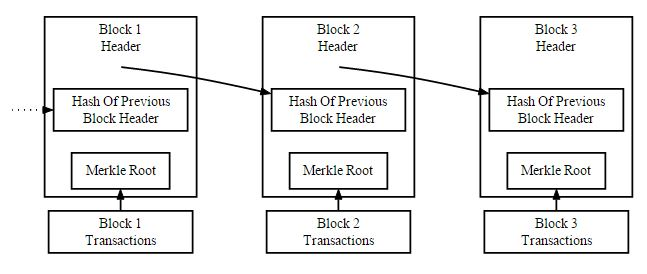
\includegraphics[width=0.85\textwidth,angle=0]{images/block-chain}
 	\caption{Verkettung von Blöcken durch Block Header Hashes}
	\label{fig:block-chain}
\end{figure}

Die Blockchain ist verteilt gespeichert. Jeder Teilnehmer hat die Möglichkeit Sie auf seinen Rechner zu speichern. Somit besteht keine zentrale Instanz, welche die Kontrolle über die Daten hat. Weiterhin gibt es keinen Single Point of Failure\footnote{Single Point of Failure: Komponente eines Systems, dessen Ausfall den Ausfall des gesamten Systems bewirkt \cite{SinglePointFailure2016}.},  \cite{CrosbyBlockChainTechnologyBitcoin2016}.

\label{subsec:konsens}
\subsection{Konsensmechanismen}

%TODO: Nodes = Teilnehmer, welche die Blockchain speichern.
Aufgrund der verteilten Datenhaltung, muss es Verfahren geben, um die Daten synchron, und auf einen Stand, auf welchen sich alle Teilnehmer geeinigt haben, zu halten. Dazu gibt es die sogenannten Konsensmechanismen, welche gleichzeitig die Unmanipulierbarkeit der Daten sicherstellen. Bevor diese erklärt werden können, muss zunächst genauer auf die Funktion des Netzwerks eingegangen werden.

%TODO: Wann Validity-Check der Transaktionen ?
Wenn ein Teilnehmer eine Transaktion ausführt, wird diese, vorausgesetzt dass sie valide ist (Genauer im nächsten Absatz erklärt), an alle Nodes (Teilnehmer, welche die Blockchain speichern) im Netzwerk weitergeleitet und im Transaktionspool aufgenommen. Dieser enthält alle noch nicht in Blöcken vorkommenden Transaktionen. Diese werden in einen neuen Block aufgenommen, und jede Node beginnt mit der Erstellung von diesem. Das Erstellen wird durch verschiedene Konsensmechaniken realisiert. Bei Bitcoin und Ethereum findet der Proof-of-Work Anwendung (Genauer im folgenden Absatz erklärt). Sobald eine Node einen Block erstellt, wird dieser im Netzwerk verteilt. Jede Node hängt ihn an ihre lokale Blockchain an, und beginnt mit der Erstellung des nächsten Blocks \cite{MAntonopoulosMasteringbitcoin2015}.

%TODO: Private und Public Key Footnode ?
%TODO: Private und Public Key Grafik
Damit eine Transaktion valide ist, muss sie bestimmte Voraussetzungen erfüllen. So muss sie unter anderen mit den Private Key des Senders signiert sein. Mittels seines Public Keys kann überprüft werden, ob wirklich er der Sender der Nachricht ist und ob die Transaktion manipuliert wurde. Dieses Verfahren wird auch in der Abbildung \ref{fig:key-signing} visualisiert. Das Signieren trägt zur Sicherheit der Blockchain bei, da ein Angreifer somit keine Transaktionen manipulieren oder im Namen eines anderen ausführen kann. In Bitcoin ist eine weitere Kondition, dass der Transaktionsersteller die zu sendenen Bitcoins besitzt \cite{AntonopoulosMasteringbitcoin2015}. In Systemen wie Ethereum und Hyperledger Fabric, in welchen eigene Programmlogik abgebildet werden kann, können weitere Konditionen festgelegt werden. So muss z.B. ein Teilnehmer die nötigen Rechte haben um eine Transaktion auszuführen \cite{AccessControlLanguage}.

%TODO: Weglassen ?
\begin{figure}[htb]
	\centering
	  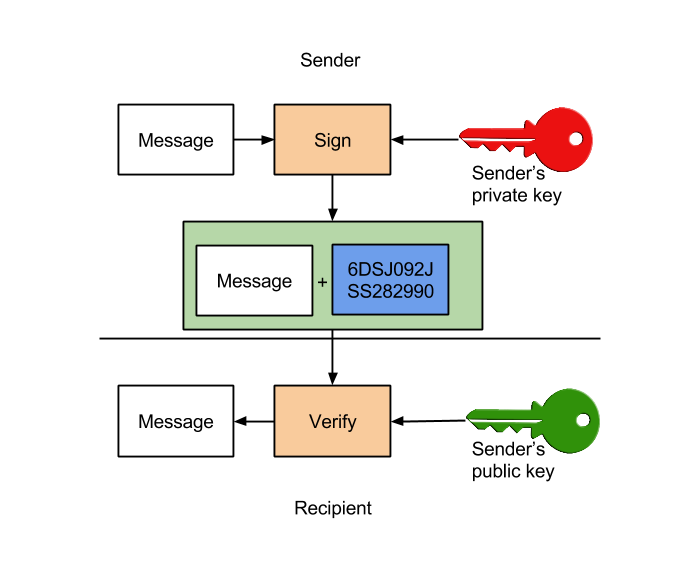
\includegraphics[width=0.7\textwidth,angle=0]{images/key-signing}
	  \caption{Signieren und Verifizieren von Nachrichten. Der Sender signiert die Nachricht mit seinen Private Key und der Empfänger kann diese mit den Public Key des Senders verifizieren.}
	  \label{fig:key-signing}
\end{figure}
	

%TODO: Zeiten für die Block-Erstellung erwähnen ?
Der Proof-of-Work ist nur einer der zur Verfügung stehenden Konsensmechanismen (Siehe Kapitel \ref{subsec:eval-konsens}). Er bedarf jedoch genauerer Erklärung, da er in aktuellen Blockchain-Implementationen vorwiegend genutzt wird. Der Proof-of-Work ist eine Art Rätsel, welches mit der Rechenleistung von Nodes gelöst werden muss, um einen Block zu erschaffen. Genauer gesagt, muss für einen Block ein Hash gefunden werden, welcher einen bestimmten Wert unterschreitet. Desto kleiner dieser ist, desto höher ist die Schwierigkeit. Um wachsender Rechenleistung und Teilnehmerzahl entgegen zu wirken, also die Zeit für die Erstellung eines Blockes ungefähr gleich zu halten, kann die Schwierigkeit angepasst werden. Dies ist aufgrund verschiedener Faktoren nötig, welche genauer im Kapitel \ref{cha:b2b-eval} erläutert werden. Um unterschiedliche Hashwerte für gleiche Blöcke zu erhalten, gibt es im Block Header eine Nonce\footnote{Nonce: Eine ``Zahlen- oder Buchstabenkombination, [...] die nur ein einziges Mal in dem jeweiligen Kontext verwendet wird''\cite{Nonce2017}.}, welche verändert wird \cite{NakamotoBitcoinPeertoPeerElectronic2008}. Alle Nodes im Bitcoin-Netzwerk benötigen im Durchschnitt 10 Minuten um einen Proof-of-Work zu erbringen \cite{AntonopoulosMasteringbitcoin2015}, bei einer Hash Rate\footnote{Hash Rate: Anzahl der in einer Zeiteinheit berechneten Hashwerte \cite{GlossarBitcoin}.} von ca. 13.000.000 TH/s (Terrahashes pro Sekunde) \cite{HashRate}. Bei Ethereum beträgt die Zeit ungefähr 14 Sekunden \cite{EthereumAverageBlockTime}, bei einer Hash Rate von ca. 150 TH/s \cite{EthereumNetworkHashRate}. Damit die Nodes eine Motivation haben, Rechenleistung für das Erstellen von Blöcken zu nutzen, erhalten sie bei Erbringung des Proof-of-Work eine Belohnung in Form von Währung \cite{NakamotoBitcoinPeertoPeerElectronic2008} \cite{EthereumWhitepaper2017}. 

Um vollständig zu verstehen, wie der Proof-of-Work funktioniert, muss das Forking erklärt werden. Wenn eine Node einen Proof-of-Work erbringt, also einen Block erstellt, wird dieser an alle anderen Nodes weitergeleitet. Im Bitcoin-Netzwerk dauert es bei einer maximalen Blockgröße von 1MB \cite{AntonopoulosMasteringbitcoin2015}, zwischen 6 und 20 Sekunden, bis ein Block mindestens 90\% aller Nodes erreicht hat \cite{BitcoinStatsb}. In dieser Zeit kann es vorkommen, dass eine weitere Node einen Block erstellt. Auch dieser wird im Netzwerk verteilt, womit 2 Versionen der Blockchain existieren: Eine endet mit Block A, und die andere mit Block B. Dies ist der sogenannte Fork. Das Netzwerk muss sich nun darauf einigen, welche der beiden Versionen beibehalten werden soll. Deshalb gilt: Die längere Blockchain ist die gültige. Die Nodes probieren an den zuerst erhaltenen Block (A oder B) einen neuen anzuhängen. Gelingt dies, ist eine der beiden Blockchains länger als die andere. Diese wird dann von allen Nodes als die richtige akzeptiert \cite{AntonopoulosMasteringbitcoin2015}. Dieser Vorgang wird auch in den Abbildungen \ref{fig:fork_1} bis \ref{fig:fork_4} dargestellt. Theoretisch ist es möglich, dass ein Fork über mehrere Blöcke bestehen muss. Die Wahrscheinlichkeit dafür ist jedoch gering, da mehrmals nacheinander mindestens 2 Nodes zur ungefähr gleichen Zeit einen Block erstellen müssen. Dies ist auch der Grund, warum Transaktionen erst als bestätigt gelten, sobald sie in einem Block stehen, welcher eine gewisse Anzahl an Nachfolgern hat. Denn erst dann ist die Sicherheit gegeben, dass die Transaktion nicht in einem Fork vorhanden ist, welcher eventuell verworfen wurde. Wie genau der Proof-of-Work das Netzwerk absichert, wird im Kapitel \ref{subsec:immutability} erklärt.


\begin{figure}[htb]
  \centering
    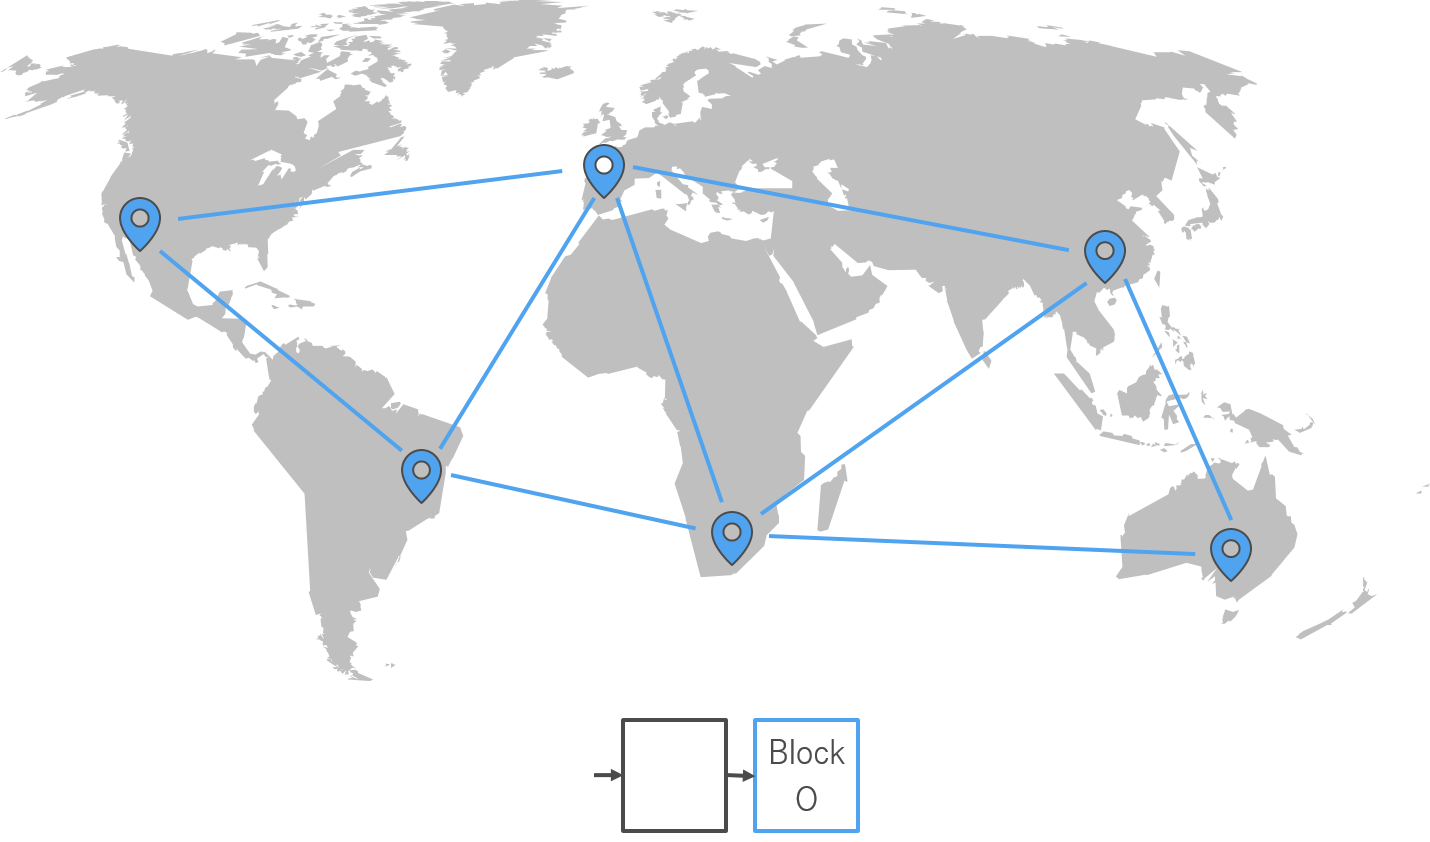
\includegraphics[width=0.95\textwidth,angle=0]{images/fork_1}
 	\caption{Fork-Visualisierung - Vor dem Fork besitzen alle Nodes Block O als letzten Block \cite{AntonopoulosMasteringbitcoin2015}.}
	\label{fig:fork_1}
\end{figure}

\begin{figure}[htb]
  \centering
	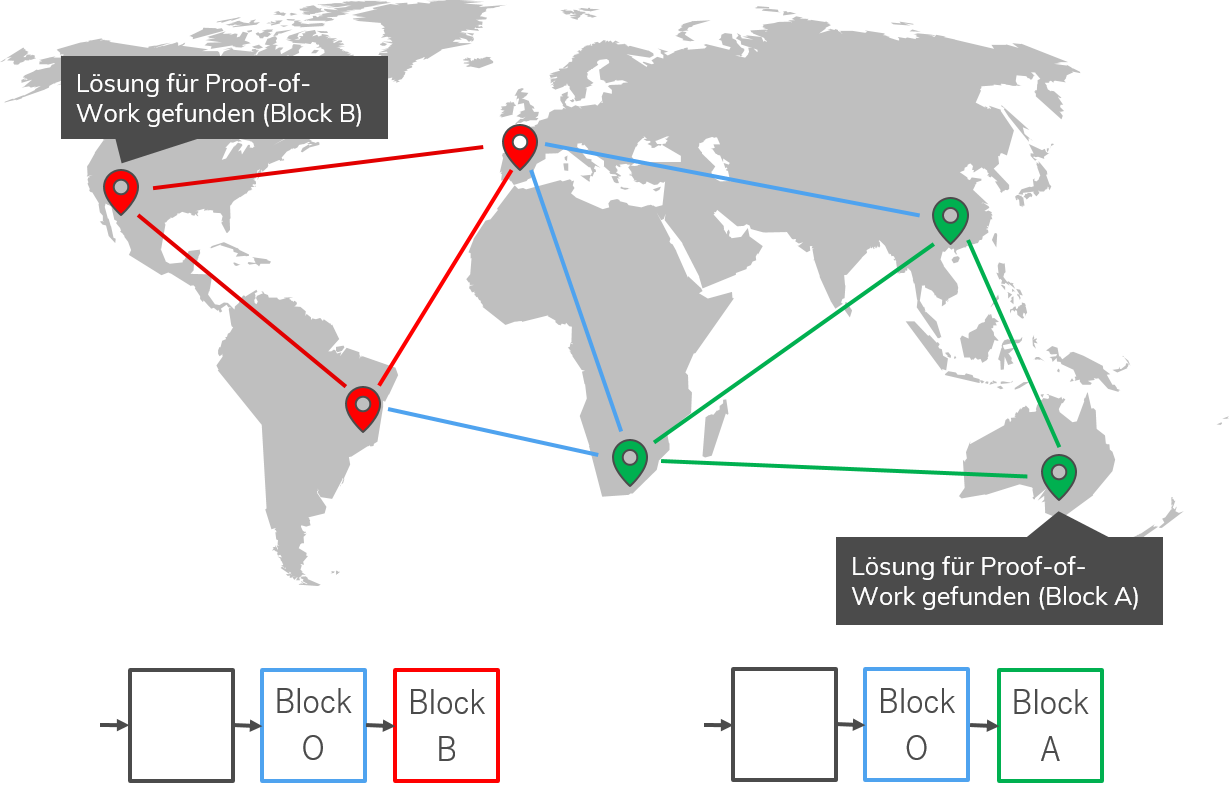
\includegraphics[width=0.95\textwidth,angle=0]{images/fork_2}
 	\caption{Fork-Visualisierung - 2 Nodes finden zur ungefähr gleichen Zeit einen Block und verbreiten ihn im Netzwerk, womit 2 Versionen der Blockchain bestehen \cite{AntonopoulosMasteringbitcoin2015}.}
	\label{fig:fork_2}
\end{figure}

\begin{figure}[htb]
  \centering
	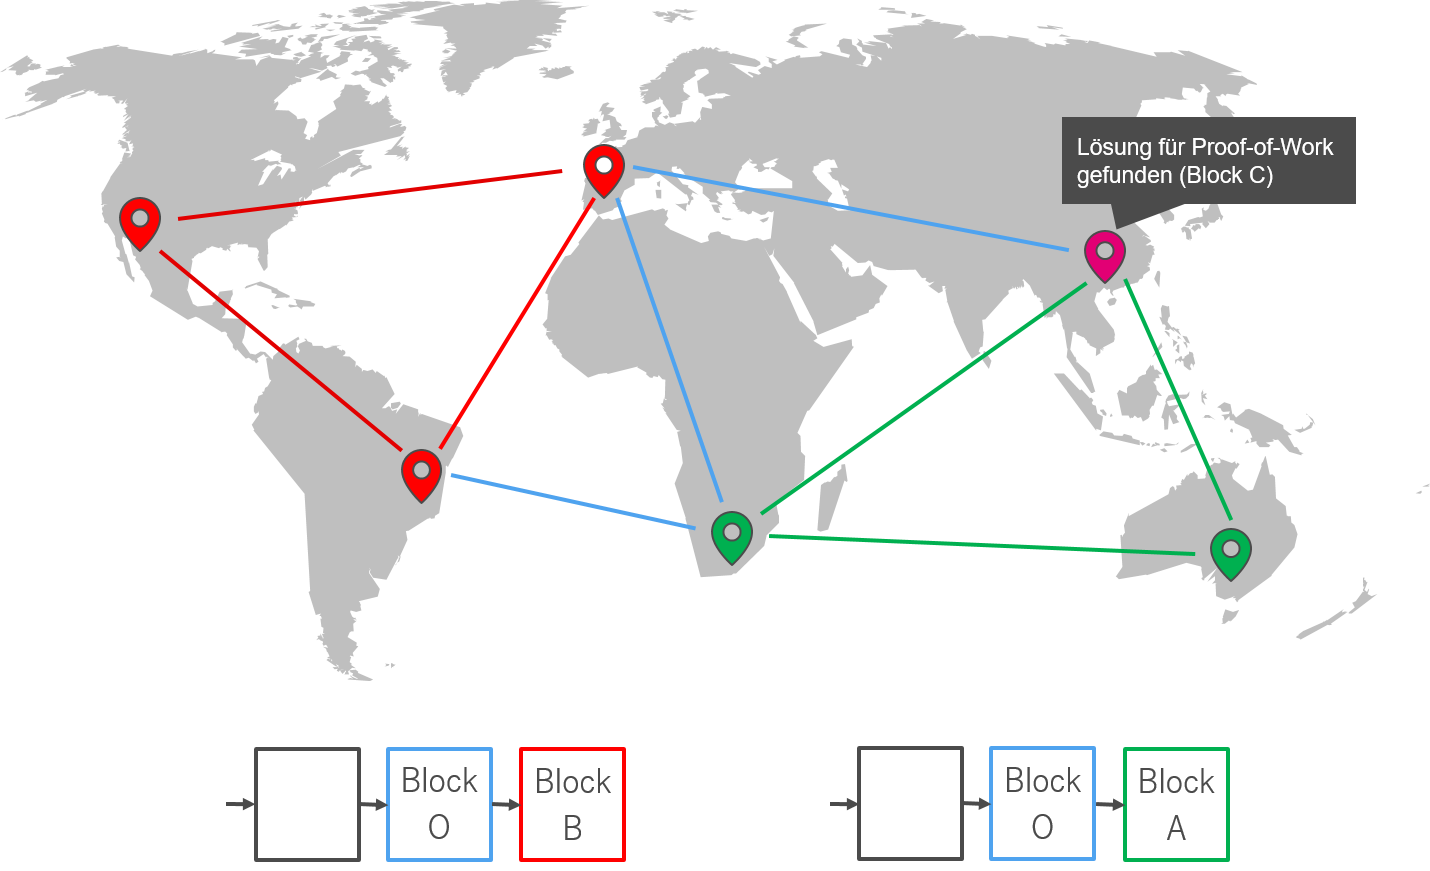
\includegraphics[width=0.95\textwidth,angle=0]{images/fork_3}
 	\caption{Fork-Visualisierung - Eine Node, welche Block A zuerst erhalten hat, hängt daran einen neuen Block C an \cite{AntonopoulosMasteringbitcoin2015}.}
	\label{fig:fork_3}
\end{figure}

\begin{figure}[htb]
  \centering
	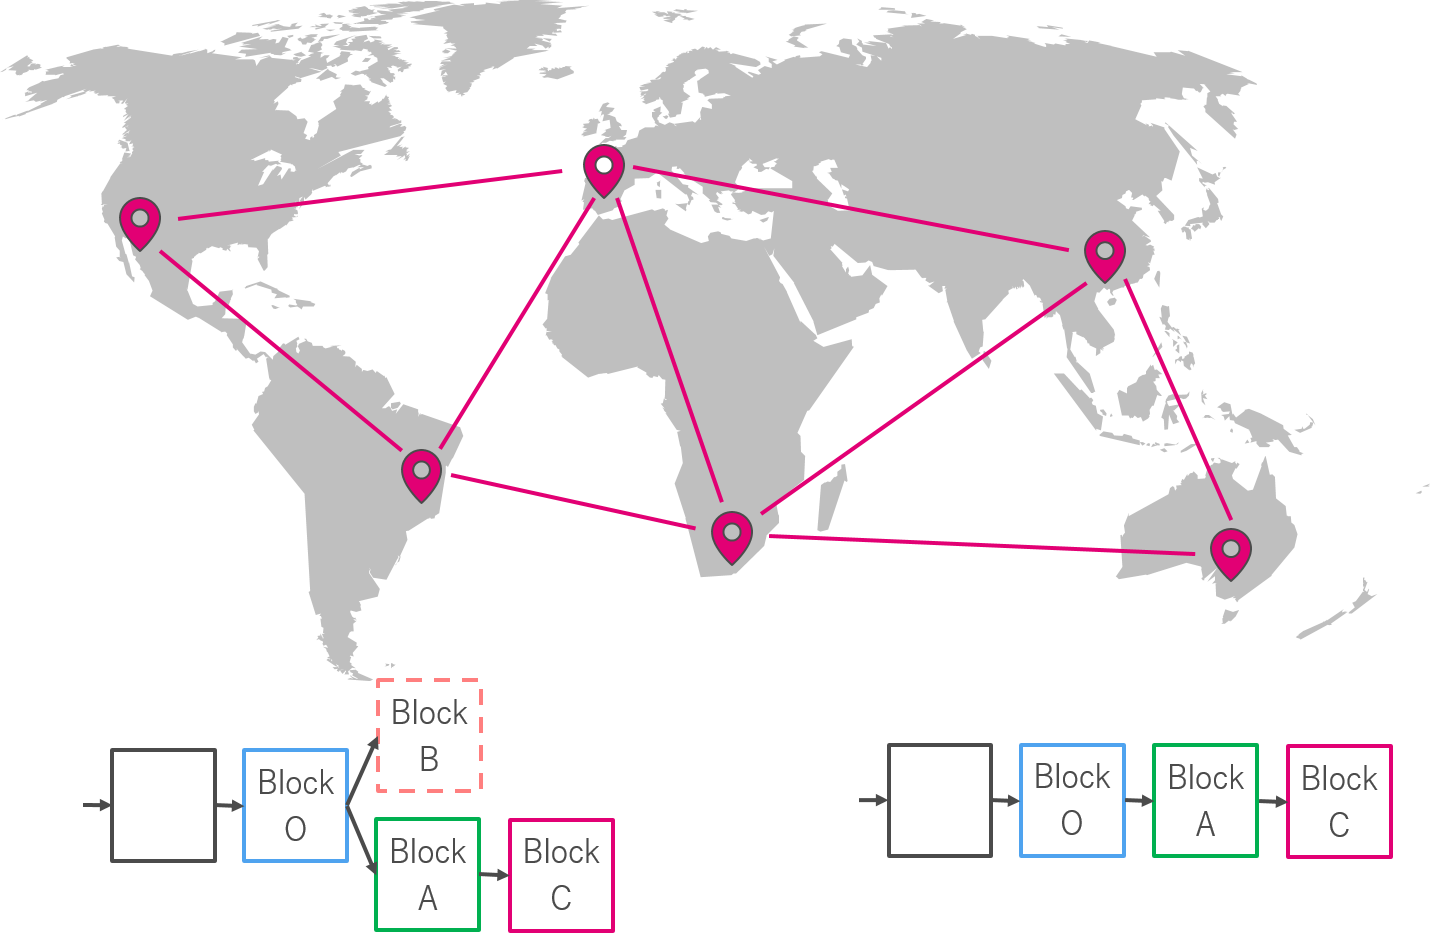
\includegraphics[width=0.95\textwidth,angle=0]{images/fork_4}
 	\caption{Fork-Visualisierung - Block C verbreitet sich im Netzwerk, rote Nodes sehen zwei Blockchains und akzeptieren die längere \cite{AntonopoulosMasteringbitcoin2015}.}
	\label{fig:fork_4}
\end{figure}

Neben dem Proof-of-Work gibt es noch weitere Konsensmechanismen, wie Proof-of-Stake, Proof-of-Authority oder Practical Byzantine Fault Tolerance \cite{SukhwaniPerformanceModelingPBFT2017a}, \cite{DeAngelisPBFTvsproofofauthority2017} . Diese werden im Kapitel \ref{subsec:eval-konsens} genauer beschrieben und analysiert.

%TODO: S.18 ZhengBlockchainChallenges: Selfish Mining Attack and following attacks
\label{subsec:immutability}
\subsection{Nichtangreifbarkeit/Immutability}
Viele Faktoren tragen zur Nichtangreifbarkeit und Unveränderlichkeit der Blockchain bei. Da alle Nodes die ausgeführten Transaktionen auf Validität prüfen, können diese nicht ohne Berechtigung, im Namen einer anderen Identität, oder mit unzureichenden Konditionen ausgeführt werden. Der wichtigste Faktor ist jedoch der genutzte Konsensmechanismus in Verbindung mit den verketteten Blöcken. Durch ihm wird sichergestellt, dass bestehende Daten nicht gelöscht oder manipuliert werden können.

%TODO: Erwähnen, dass entfernte Transaktionen zurück in den Transaktionspool gehen ? Das würde bedeutete, um eine Transaktion für immer aus den Blöcken rauszuhalten, muss der Angreifer diese in jeden Block absichtlich nicht aufnehmen (Er muss jeden weiteren Block erstellen), oder eine im Konflikt stehende Transaktion in einen Block aufnehmen (Double-Spending-Attacke bei Kryptowährungen), oder eine beliebige andere Transaktion muss die entfernte Transaktion invalide machen (z.B. kann nur ausgeführt werden wenn ein Vertrag noch nicht akzeptiert wurde)
Ein Beispiel dafür kann am Proof-of-Work gezeigt werden. Ein Angreifer probiert eine Transaktion aus einen bestehenden Block zu entfernen. Dazu würde er die Transaktion bei seiner lokalen Blockchain entfernen. Nun ist jedoch der Hash des Blockes sowie der Block selber nicht valide und würde von keiner Node akzeptiert werden. Der Angreifer muss also erneut einen Proof-of-Work für den manipulierten Block erbringen. Dies wäre für eine Einzelperson jedoch Zeitaufwändig, wenn man bedenkt, das extra für diesen Zweck produzierte Hardware eine Hash Rate von bis zu 13,5 TH/s erreicht \cite{Mining?LearnBitcoinmining}. Dies  Wenn der manipulierte Block nun noch Nachfolger hat, muss aufgrund des neuen Hashes auch für diese der Proof-of-Work erbracht werden. Hinzu kommt, dass die Blockchain des Angreifers erst von allen Nodes akzeptiert wird, wenn sie länger ist. Er müsste also schneller als das gesamte Bitcoin-Netzwerk Blöcke erschaffen können.  Dies ist nur möglich, wenn er 51\% der Rechenleistung des Netzwerks besitzt. Deshalb wird dieser Angriff auch 51\%-Angriff genannt \cite{SwanBlockchainblueprintnew2015} \cite{EthereumWhitepaper2017}.

An dieser Stelle sollte erähnt werden, dass auch wenn ein 51\%-Angriff erfolgt, die Angriffsmöglichkeiten beschränkt sind. Der Angreifer kann keine unvaliden Transaktionen sowie Blöcke erstellen. Ihm ist es möglich DoS-Angriffe auszuführen indem er verhindert das bestimmte Transaktionen in Blöcke aufgenommen werden. Genau so kanner die Historie der Daten verändern, indem er eine Transaktion aus einem Block entfernt und diese nicht erneut in einen Block aufnimmt. Im Falle von Kryptowährungen gibt es außerdem die sogenannte Double-Spending-Attacke. Diese funktioniert folgendermaßen: Ein Angreifer sendet z.B. Bitcoins an einen Händler. Dieser wartet auf die Bestätigung der Transaktion in einen Block sowie auf nachfolgende Blöcke. So stellt er sicher, dass die Transaktion nicht in einem eventuell verworfenen Fork stand. Erst dann versendet er die Ware. Anschließend ersetzt der Angreifer die Transaktion durch eine Zahlung an sich selber und erstellt die längere Blockchain, womit der Händler letztendlich kein Geld erhalten hat \cite{EthereumWhitepaper2017}. Auch zu bedenken ist, dass ein Nutzer mit 51\% der Rechenleistung wenig Motivation hat Angriffe auszuführen, da er für jeden erstellten Block Kryptowährung als Belohnung erhält. Der Wert der Kryptowährung würde sinken, wenn Angriffe auf die Blockchain entdeckt werden. Deshalb besteht für die sogenannten Miner eine Motivation, ehrlich zu arbeiten \cite{AntonopoulosMasteringbitcoin2015}. 

%TODO: Tabelle mit Vergleich der Typen ?
\section{Blockchaintypen}
Es gibt 3 Typen von Blockchains, welche die zugelassenen Teilnehmer bestimmen. Bisher wurden nur Public Blockchain-Anwendungen, wie Bitcoin und Ethereum erwähnt. In diesen gibt es keine Teilnehmerbeschränkungen, jeder kann am Netzwerk teilnehmen und die Blockchain öffentlich einsehen. Anders ist dies bei Permissioned (oder auch Consortium \cite{BenHamidaBlockchainEnterpriseOverview2017}) und Private Blockchains. Die beiden Begriffe werden in einigen wissenschaftlichen Arbeiten gleichgesetzt (Siehe \cite{Gramolidangerprivateblockchains2016}, \cite{PongnumkulPerformanceAnalysisPrivate2017a}, \cite{LiScalablePrivateIndustrial2017}). Hier folgt jedoch eine Unterscheidung. Dabei ist eine Private Blockchain, eine Blockchain welche nur von einen Nutzer verwendet wird. Da eine solche Anwendung keinen Sinn macht, da keine Vorteile der Blockchain genutzt werden können, wird darauf nicht genauer eingegangen. Interessanter sind Permissioned Blockchains, an welchen nur zugelassene Nutzer teilnehmen dürfen. Nur diese sind berechtigt, Transaktionen auszuführen und die Daten einzusehen \cite{LiScalablePrivateIndustrial2017}. Dies bietet sich vor allem bei B2B-Anwendungen an, welche von verschiedenen Unternehmen genutzt werden sollen. In diesen kann es aufgrund von z.B. sensiblen Daten nötig sein, das nur bestimmte Parteien Zugriff auf die Blockchain haben.
An dieser Stelle sollte auch erwähnt werden, dass es möglich ist Blockchain-Implementationen wie z.B. Ethereum als Permissioned Blockchain zu nutzen \cite{MercuryProtocolHowCreateYour2017}.

\label{subsec:use-cases}
\section{Exemplarische Anwendungsfälle}
%TODO: Gartner Hype Cycle erwähnen ?
Die Blockchain wird als revolutionäre Technologie angepriesen (Siehe \cite{TapscottBlockchainRevolutionWieTechnologie2016}). Trotzdem ist es wichtig zu wissen, für welche Zwecke sie wirklich geeignet ist. Grundsätzlich macht eine Blockchain Sinn, wenn mehrere Parteien, welche sich nicht vertrauen, mit einen System interagieren wollen, welches von keiner dritten zentralen Instanz verwaltet wird \cite{WustyouneedBlockchain2017}. Um eine bessere Vorstellung zu solchen Anwendungen zu erhalten, werden im Folgenden verschiedene Exemplarische Anwendungsfälle genannt und beschrieben.

Der erste Anwendungsfall, mit welchen die Blockchain-Technologie auch entstanden ist, sind Kryptowährungen. Mit Ihnen ist es möglich Geld zwischen beliebigen Parteien zu übertragen, ohne dass die Transaktionen von einer eventuell nicht vertrauenswürdigen Bank oder ähnlichem kontrolliert und verwaltet werden \cite{SwanBlockchainblueprintnew2015}.

%TODO: Smart Contracts erwähnen ?
Weitere Anwendungsfälle ergeben sich mit der Möglichkeit Programmlogik auf der Blockchain abzubilden. So können beispielsweise dezentrale Online-Wahlen realisiert werden. Die Stimmen würden in der Blockchain gesammelt werden, und können so letztendlich nicht mehr von z.B. einer korrupten Regierung manipuliert werden \cite{CastorEthereumVotingScheme2017}. 

%TODO: SoldatosWhatDoes Supply Chain Explanation
%TODO: S.3 WustYouNeed Supply Chain Explanation
%TODO: S.3 Korpela Supply Chain Problems (?)
Ein weiterer Anwendungsfall, insbesondere für den B2B-Bereich, wäre Supply Chain Management. Über eine digitale Lieferkette sollen Material- und Informationsflüsse zu Produkten und Dienstleistungen aufgebaut und verwaltet werden \cite{KriegerDefinitionSupplyChain}. Dies erlaubt Unternehmen das automatisieren von Prozessen und das verbesserte reagieren auf Ereignisse (z.B. Lieferverspätungen). Weiterhin ist es dem Unternehmen möglich, dem Kunden exakt aufzuzeigen wo es und seine Unterprodukte produziert wurden. In klassischen B2B-Anwendungen müsste jedes Unternehmen, welches ein Teil der Supply Chain ist, die relevanten Daten durch z.B. APIs\footnote{API: Schnittstelle zur Anwendungsprogrammierung\cite{Programmierschnittstelle2017}} bereitzustellen. Dies bedeutet Aufwand, da diese erstmal entwickelt werden müssen. Weiterhin müsste ein System von all diesen unterschiedlichen Schnittstellen die Daten abfragen und in einem System zusammenführen um die Supply Chain zu erstellen. Diese müssten dann abgefragt werden um die Supply Chain zu erstellen. Aufgrund dieses Aufwandes werden oft Dritte eingestellt, welche sich um den Aufbau und um die Datenintegration der Supply Chain kümmern. Den Aufwand, sowie die eventuell nicht vertrauenswürdige dritte Partei könnte man durch die Nutzung der Blockchain überspringen. In dieser könnte jedes Unternehmen die relevanten Daten speichern, ohne das aufwändige Erstellen von Schnittstellen. Die Supply Chain wäre direkt in der Blockchain vorhanden, und kein Unternehmen muss Datenmanipulation oder ähnliches befürchten \cite{KorpelaDigitalSupplyChain2017}.

%TODO: S.1 DecentralizedMarketplace: Online Services collecting our data --> Need for new 
Auch dezentrale Märkte sind für B2B-Anwendungen interessant. Der zentrale Marktplattformbetreiber, wie z.B. Ebay oder Amazon, welcher persönliche Informationen speichert und Gebühren für den Verkauf von Artikeln verlangt, wäre hinfällig. Nutzer könnten Waren untereinander verkaufen, während die Blockchain als Notar für den Warenaustausch dient \cite{BenHamidaBlockchainEnterpriseOverview2017}.

%TODO: Bike-Sharing weglassen ?
Ein weiteres Beispiel wären Blockchain Sharing-Systeme. So könnte ein dezentrales Fahrradleihsystem aufgebaut werden. Nutzer würden mit ihrem Smartphone, über ihre in der Blockchain hinterlegte Identität (Im Falle von z.B. Ethereum die Wallet-Adresse\footnote{Wallet: Speichert z.B. bei Ethereum und Bitcoin den Private Key des Nutzers und wird z.B. als Adresse für Zahlungen genutzt \cite{BlockchainWallet}.}), das Fahrrad entsperren. Dieser erkennt automatisch die gefahrene Distanz sowie die Nutzungsdauer. Über einen Smart Contract würde anschließend die automatische Zahlung erfolgen. Neben der Automatisierung besteht der Vorteil, dass mehrere Unternehmen oder auch Privatpersonen Leihfahrräder anbieten können, ohne dass sie einer zentralen Instanz mit der Verwaltung vertrauen müssen \cite{BlockchainBikes}, \cite{FischerIoTBlockchain}.  

%\label{sec:bc-problems}
%TODO: Aus Grundlagenkapitel entfernen und zu Kapitel 5 (B2B-Evaluierung) verschieben
%\section{Probleme für den B2B-Bereich}
%Die Blockchain bringt gewisse Probleme mit sich, welche verschieden große Auswirkungen auf B2B-Anwendungen haben können. Diese werden im folgenden kurz analysiert.

%\subsection{Skalierbarkeit}

%\subsection{title}

%Private Transaktionen

%Proof-of-Work Unsicherheit und Energieverbrauch

%\begin{itemize}
%	\item Probleme erwähnen
%   \item Probleme genauer auf den B2B-Bereich beziehen
%   \item Blockerstellungszeit --> Warum konstant, 10 Minuten etc. ?
%\end{itemize}
